% KMP fallback figure
\ifdefined\includetikz\relax \else
%\documentclass{standalone}
\documentclass{article}
\usepackage{tikz}
\usepackage{amsmath}
\usetikzlibrary{matrix,positioning}
\begin{document}
\fi

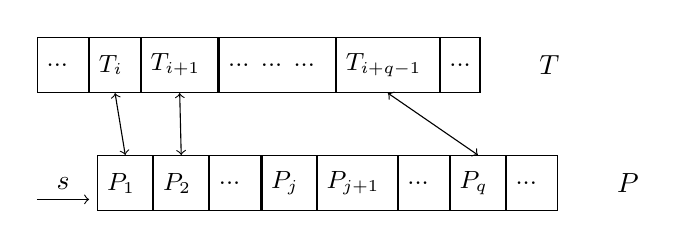
\begin{tikzpicture}[
scale=0.5,
array/.style={matrix of nodes,
              font=\small,
              minimum height=7mm,
              %text width=2mm,
              nodes={draw, align=center, anchor=south},
              nodes in empty cells
              }]

% T
\matrix[array] (mytext) {
... & $T_i$ & $T_{i+1}$ & ... ... ... & $T_{i+q-1}$ & ...\\};
\node[right=0.5cm of mytext] {$T$};

% P
\matrix[array,
  anchor=west] at ([yshift=-3cm, xshift=-0.7cm]mytext-1-2) (myptn) {
$P_1$ & $P_2$ & ... & $P_j$ & $P_{j+1}$ & ... & $P_q$ & ... \\};
\node[right=0.5cm of myptn] {$P$};

% offset s
\draw[->] ([yshift=-2.7cm]mytext-1-1.south west) -- node[above] {$s$} ([yshift=-2.7cm]mytext-1-1.south east);

% matches chars so far.
\foreach \i/\j in {2/1, 3/2, 5/7} {
  \draw[<->] (mytext-1-\i.south) -- (myptn-1-\j.north);
}

\end{tikzpicture}

\ifdefined\includetikz\relax \else
\end{document}
\fi
